\chapter{Vorüberlegungen}
Zu Beginn der Studienarbeit mussten einige Vorüberlegungen getätigt werden:
\begin{itemize}
  \item Es musste ein Datenmodell erstellt werden, welches die Struktur der Datenbank beschreibt.
  \item Es mussten alle zu diesem Zeitpunkt bereits bekannten Aufgaben festgehalten werden, um sich
  einen Überblick über den Funktionsumfang und Arbeitsaufwand zu verschaffen.
\end{itemize}
Aus den so erhaltenen Aufgaben und den Funktionalitäten, die das Projekt am Ende bieten sollte, sollte ein Konzept zum Design einer passenden Oberfläche erstellt werden. 

\section{Datenmodell}
Das Datenmodell wurde früh entwickelt und sollte als Grundlage dienen, um die Datenstruktur der Datenbank implementieren. 
Dabei ist es wichtig Zeit in das Datenmodell zu investieren, da das Datenmodell als fundamentale Grundlage dient und große Änderungen daran später zeitaufwändige Folgen haben würden.
Dabei wurde ein eine relationale Datenbank gewählt und versucht, das Datenmodell nach den Prinzipien der Theorie der realtionalen Datenbanken aufzubauen.
Dementsprechend wurde die Tabellenstruktur in dritter Normalform aufgebaut.\\
Im Verlauf der Studienarbeit mussten dennoch Änderungen am Datenmodell vorgenommen werden, jedoch waren diese nur kleine Änderungen, wie z.B. das Hinzufügen einer Spalte innerhalb einer Tabelle.
Dies lässt den Schluss zu, dass die zu Beginn investierte Zeit in das Datenmodell und die Gespräche und Diskussionen zu Beginn hierzu sinnvoll investierte Zeit waren.

\begin{landscape}
\begin{figure} [!htb]
	\begin{center}
		  \begin{tabular}{@{}r@{}}
			{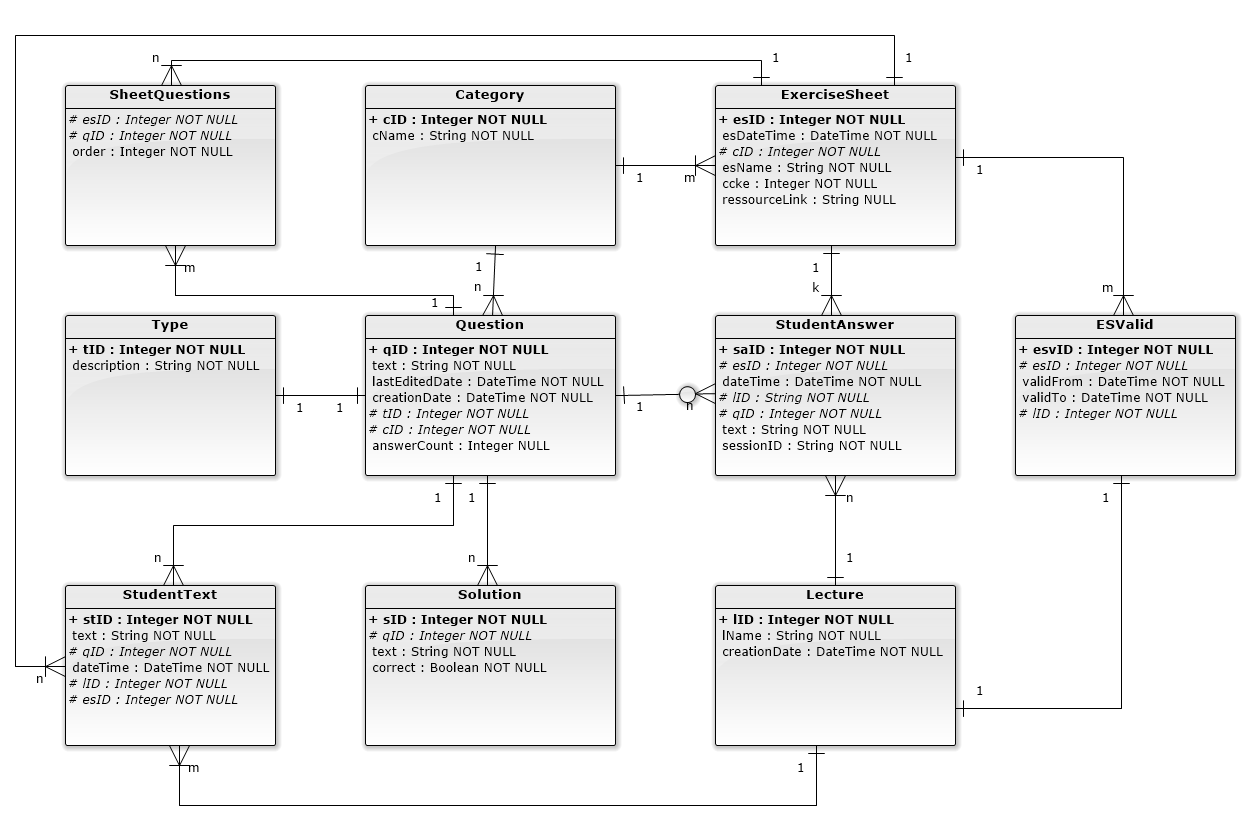
\includegraphics[height=37em]{images/Entityrelationshipdiagram.png}}\\
 	 	 \end{tabular}
		\caption{Datenmodell LeMon + CCKE}
		\label{fig:Datenmodell}
	\end{center} 
\end{figure}

\end{landscape}




\section{Erklärung des Datenmodells}

In der DB-Tabelle \textbf{Category} werden die Namen der erstellten Kategorien
abgespeichert.

Die DB-Tabelle \textbf{Type} enthält die Namen der verschiedenen Fragentypen.

In der DB-Tabelle \textbf{Lecture} sind die Namen der erstellten Vorlesungen
enthalten.

In die DB-Tabelle \textbf{Question} können die erstellten Fragen abgespeichert werden.
Zudem können über sie Verknüpfungen zu den Tabellen \emph{Type} und
\emph{Category} hergestellt werden. Das Attribut \emph{answerCount} gibt die
Anzahl der geforderten Antworten für Aufzählaufgaben an.

Die DB-Tabelle \textbf{Solution} dient zur Abspeicherung von allen
Musterlösungen zu den erstellten Fragen sowie die IDs der zugehörigen Fragen.
Das Attribut \emph{correct} gibt dabei an, ob es sich bei einer Multiple-Choice
Antwort um eine korrekte oder eine falsche Antwort handelt.

In der DB-Tabelle \textbf{ExerciseSheet} werden die Namen, sowie die
Erstelldaten der erstellten Aufgabenblätter abgespeichert. Das Attribut
\emph{ccke} gibt an, ob es sich um ein Arbeitsblatt für \gls{CCKE} handelt oder
nicht. Das Attribut \emph{ressourceLink} ist für \gls{CCKE} notwendig und hat
keinerlei Relevanz für \gls{LeMon}. Zudem gibt es eine ID zur Verknüpfung der
Kategorie.

Über die DB-Tabelle \textbf{SheetQuestions} kann eine Verknüpfung zwischen
Fragen und Aufgabenblättern hergestellt werden. Zusätzlich ist durch das
Attribut \emph{order} die Reihenfolge der Fragen auf dem Aufgabenblatt
festgelegt.

Die DB-Tabelle \textbf{ESValid} beschränkt den Zeitraum der Gültigkeit eines
Aufgabenblattes. Ebenso wird hierrüber eine Verknüpfung zwischen Vorlesungen und
Aufgabenblättern hergerstellt werden.

In der DB-Tabelle \textbf{StudentAnswer} werden alle Antworten der Studenten
für Multiple-Choice und Aufzählaufgaben abgespeichert. Zusätzlich wird ein Zeitstempel in Form
von Datum und Uhrzeit sowie eine Session ID abgespeichert. Die Session ID soll
lediglich zur eindeutigen Zuordnung einer Antwort zu einer einzelnen Person,
jedoch nicht zu einer eindeutig identifizierbaren dienen. Dabei existieren
Verknüpfungen zu einem Aufgabenblatt, zu einer Frage und zu einer Vorlesung.

Die DB-Tabelle \textbf{StudentText} beinhaltet alle Freitextantworten der
Studenten für Freitextfragen.




\section{Mapping von Use-Case zu Datenmodell}

\begin{table}[h]
	\begin{tabular}{|p{3cm}|p{11.06cm}|}
	\hline
		\textbf{Zugehöriger Use Case}                 &   \emph{UC1: Frage mit Musterlösungen anlegen} \prettyref{uc:UC1}     \\ \hline
		\textbf{Beteiligte Tabellen}      &     Question, Type, Category, Solution    \\ \hline
		\textbf{Vorbedingung}              &     Alle benötigten Daten wurden eingegeben    \\ \hline
		\textbf{Ablauf}              &   
			\begin{enumerate}
			  \item Es wurden schon beim Aufrufen des „Frage erstellen“ Formular, die Kategorien und Typen mit ihren IDs geladen
			  \item Beim abschicken des Formulars wird ein neuer Eintrag in die Tabelle „Question“ erstellt mit einer automatisch hochzählenden ID (qID), der Kategorie (cID) und Typen (tID), dem jetzigen Datum mit Uhrzeit (creationDate und lastEditedDate), und der eigentlichen Frage (text).
			  \item Die dazu gehörigen Antworten werden in die „Solution“ Tabelle gespeichert mit einer automatisch hochzählenden unique ID (sID), der dazu gehörigen Fragen ID (qID), der Antwort selbst (text) und ob es sich um eine korrekte oder falsche Antwort handelt (correct) [wichtig für Multiple-Choice]
			\end{enumerate}
		\\ \hline
		\textbf{Erweiterungen}              &        \\ \hline 
	\end{tabular}
	\caption{Mapping der Tabellen zu Use Case 1}
\end{table}\FloatBarrier

\begin{table}[h] 
	\begin{tabular}{|p{3cm}|p{11.06cm}|}
	\hline
		\textbf{Zugehöriger Use Case}                 &     \emph{UC2: Kategorie anlegen} \prettyref{uc:UC2}    \\ \hline
		\textbf{Beteiligte Tabellen}      &     Category    \\ \hline
		\textbf{Vorbedingung}              &    Alle benötigten Daten wurden eingegeben     \\ \hline
		\textbf{Ablauf}              &    Beim Abschicken des Formulars wird in der Tabelle „Category“ ein neuer Eintrag erstellt mit automatisch hochzählender ID (cID) und dem Namen der Kategorie (cName)
		\\ \hline
		\textbf{Erweiterungen}              &         \\ \hline
	\end{tabular}
	\caption{Mapping der Tabellen zu Use Case 2}
\end{table}\FloatBarrier

\begin{table}[h]
	\begin{tabular}{|p{3cm}|p{11.06cm}|}
	\hline
		\textbf{Zugehöriger Use Case}                 &    \emph{UC3: Vorlesung anlegen} \prettyref{uc:UC3}     \\ \hline
		\textbf{Beteiligte Tabellen}      &     Lecture    \\ \hline
		\textbf{Vorbedingung}              &    Alle benötigten Daten wurden eingegeben     \\ \hline
		\textbf{Ablauf}              &   Beim Abschicken des Formulars wird in der Tabelle „Lecture“ ein neuer Eintrag erstellt mit automatisch hochzählender ID (cID) und dem Namen der Vorlesung (lName) \\ \hline
		\textbf{Erweiterungen}              &         \\ \hline
	\end{tabular}
	\caption{Mapping der Tabellen zu Use Case 3}
\end{table}\FloatBarrier

\begin{table}[h]
	\begin{tabular}{|p{3cm}|p{11.06cm}|}
	\hline
		\textbf{Zugehöriger Use Case}                 &    \emph{UC4: Arbeitsblatt anlegen} \prettyref{uc:UC4}     \\ \hline
		\textbf{Beteiligte Tabellen}      &    ExcerciseSheet, SheetQuestions     \\ \hline
		\textbf{Vorbedingung}              &    Alle benötigten Daten wurden eingegeben     \\ \hline
		\textbf{Ablauf}              &   
			\begin{enumerate}
			  \item Beim Abschicken des Formulars mit dem Button „Arbeitsblatt anlegen“ wird in der Tabelle „ExcerciseSheet“ ein neuer Eintrag erstellt mit automatisch hochzählender unique ID (esID), dem Namen des Arbeitsblattes (esName) und dem Zeitpunkt der Erstellung (esDateTime)
			  \item In der Tabelle SheetQuestions wird für jede, dem Arbeitsblatt hinzugefügte, Frage ein Eintrag mit der esID und der ID der hinzugefügten Frage (qID)  eingefügt.
			\end{enumerate}
		\\ \hline
		\textbf{Erweiterungen}              &     Einstellen, wie lange Arbeitsblatt valid ist -> theoretisch auch über Button „aktiv machen“ und „sperren“ möglich.    \\ \hline
	\end{tabular}
	\caption{Mapping der Tabellen zu Use Case 4}
\end{table}\FloatBarrier

\begin{table}[h]
	\begin{tabular}{|p{3cm}|p{11.06cm}|}
	\hline
		\textbf{Zugehöriger Use Case}                 &     \emph{UC5: Antworten abschicken} \prettyref{uc:UC5}    \\ \hline
		\textbf{Beteiligte Tabellen}      &     Questions, StudentAnswer, Solution, StudentText    \\ \hline
		\textbf{Vorbedingung}              &    Alle benötigten Daten wurden eingegeben     \\ \hline
		\textbf{Ablauf}              &   
			\begin{enumerate}
			  \item Bei jeder gegebenen Antwort wird überprüft, ob es sich um eine Multiple-Choice-Frage oder um eine Freitext-Frage handelte (anhand der cID aus der Questions-Tabelle)
			  \item Abhängig von Fragetyp
			  \begin{enumerate}
			    \item Es handelt sich um eine Multiple-Choice-Antwort:
			    	\begin{enumerate}
					    \item Es wird in der Tabelle StudentAnswer ein Eintrag mit einer fortlaufenden ID (saID), der ID des Arbeitsblattes (esID), der VorlesungsID (lID), der FragenID (qID), der AntwortID (sID in der Spalte text), der SessionID seiner aktuellen Session und dem aktuellen Datum (dateTime) hinzugefügt
			  		\end{enumerate}
			  	\item Es handelt sich um eine Aufzähl-Antwort:
			    	\begin{enumerate}
					    \item Es wird in der Tabelle StudentAnswer ein Eintrag mit einer fortlaufenden ID (saID), der ID des Arbeitsblattes (esID), der VorlesungsID (lID), der FragenID (qID), dem Antworttext (text), der SessionID seiner aktuellen Session und dem aktuellen Datum (dateTime) hinzugefügt
			  		\end{enumerate}
			    \item Es handelt sich um eine Freitext-Antwort
				    \begin{enumerate}
					    \item In die Tabelle StudentText wird ein Eintrag mit einer fortlaufenden ID (stID), dem Text der Antwort, der ArbeitsblattID (esID), der VorlesungsID (lID), der FragenID (qID) und dem aktuellen Datum (dateTime) hinzugefügt.
				 	 \end{enumerate}
			  \end{enumerate}
			\end{enumerate}
		\\ \hline
		\textbf{Erweiterungen}              &         \\ \hline
	\end{tabular}
	\caption{Mapping der Tabellen zu Use Case 5}
\end{table}\FloatBarrier

\begin{table}
	\begin{tabular}{|p{3cm}|p{11.06cm}|}
	\hline
		\textbf{Zugehöriger Use Case}                 &     \emph{UC6: Auswertung des Arbeitsblattes} \prettyref{uc:UC6}    \\ \hline
		\textbf{Beteiligte Tabellen}      &    SheetQuestions, Question, StudentAnswer, StudentText     \\ \hline
		\textbf{Vorbedingung}              &         \\ \hline
		\textbf{Ablauf}              &   
			\begin{enumerate}
			  \item Zu jeder der Vorlesung und dem ausgewählten Arbeitsblatt werden die zugehörigen Fragen abgerufen.
			  \item Abhängig von Fragetyp
			  \begin{enumerate}
			    \item Es handelt sich um eine Multiple-Choice-Antwort:
				    \begin{enumerate}
					    \item Aus der Tabelle „studentAnswer“ werden nacheinander alle zur in der Vorlesung (lID) und dem Arbeitsblatt zugehörigen (esID) Frage (qID) die Antworten abgerufen und prozentual dargestellt, wie viele korrekt, falsch und nicht beantwortet wurden.
				 	\end{enumerate}
			    \item Es handelt sich um eine Freitext-Antwort
				    \begin{enumerate}
					   	\item Aus der Tabelle studentText werden zehn zufällige Antworten ausgewählt und nacheinander präsentiert.
				  	\end{enumerate}
			  \end{enumerate}
			\end{enumerate}
		\\ \hline
		\textbf{Erweiterungen}              &    Anzahl der ausgegebenen Freitext-Antworten variabel machen     \\ \hline
	\end{tabular}
	\caption{Mapping der Tabellen zu Use Case 6}
\end{table}\FloatBarrier

\section{Funktionsumfang}
Der letztendliche Funktionsumfang war zu Beginn des Projektes zwar grob klar, wie in Projekten in Unternehmen war es jedoch auch so, dass sich der Kunde gewisse Dinge später anders vorgestellt hat oder gar neue Wünsche für Funktionen äußerte.
Darauf muss man dynamisch agieren und neue Dinge während der Projektphase hinzufügen oder bestehende gegebenenfalls zu überarbeiten.
Für die wichtigsten Funktionalitäten des Projektes, wurden Use-Cases aufgestellt.

\section{Darstellung der Oberfläche}
Anhand der gesammelten Anforderungen hinsichtlich Funktionalitäten, wurden einige Oberflächen schon weitestgehend definiert. 
Als Beispiel sei hier die Funktion 'Frage erstellen' genannt, bei der gewisse Eingabefelder vorgegeben warem um den Fragentyp und -text festzulegen.
Die letztendlichen Anordnungen wurden dann in direkten Gesprächen mit dem Kunden geklärt.